%
% hardware.tex
%
% Copyright The SLCam Contributors.
%
% SLCam Documentation
%
% This work is licensed under the Creative Commons Attribution-ShareAlike 4.0
% International License. To view a copy of this license,
% visit http://creativecommons.org/licenses/by-sa/4.0/.
%

%
% \brief Hardware project chapter.
%
% \author Gabriel Mariano Marcelino <gabriel.mm8@gmail.com>
%
% \version 0.3.0
%
% \date 2021/04/02
%

\chapter{Hardware} \label{ch:hardware}

This chapter presents a description of the hardware project of the SLCam payload. As the primary reference, a block diagram can be seen in \autoref{fig:block-diagram}. Also, a 3D model of both sides of the PCB\nomenclature{\textbf{PCB}}{\textit{Printed Circuit Board}} is available in \autoref{fig:slcam-views}.

\begin{figure}[!ht]
    \begin{center}
        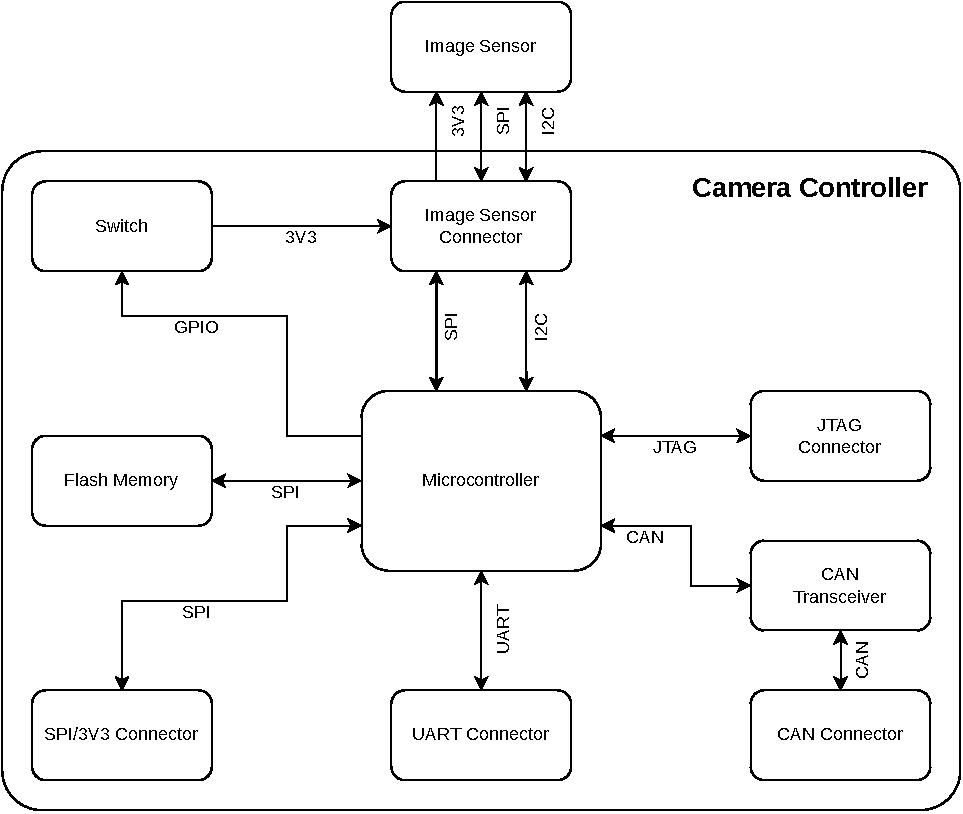
\includegraphics[width=0.8\textwidth]{figures/block-diagram.pdf}
        \caption{Block diagram of the SLCam hardware.}
        \label{fig:block-diagram}
    \end{center}
\end{figure}

The following sections present a further description of the hardware project.

\section{Specifications}

The SLCam has the image sensor module Arducam Mini 2MP Plus, one microcontroller (STM32F103C8T6) that run at a clock of \textcolor{red}{here}, a RAM of 20 kB (SRAM), a flash memory of \textcolor{red}{64 or 128KBytes}. The SLCam also has a CAN Transceiver, a switch and many connectors such as CAN connector, JTAG, SPI/3V3 and one for the image sensor.

\subsection{Image Sensor Connector}
\begin{itemize}

        \item \textbf{Sensor type}: RGB
        \item \textbf{Pixel size}: 2,2 $\times$ 2,2 $\mu$m
        \item \textbf{Max. Resolution}: 1600 $\times$ 1200 px
        \item \textbf{Field of View (FoV)}: 68$^{\circ}$ (6 mm) \textcolor{red}{TBC}
        \item \textbf{Storage}: 16 MB (Flash NOR)
        \item \textbf{Power supply}: 3V3 @ 140 mA \textcolor{red}{TBC}
        \item \textbf{Interfaces}:
            \begin{itemize}
                \item \textbf{Control/Data}: SPI and/or CAN
                \item \textbf{Debug}: UART
                \item \textbf{Programming}: JTAG
            \end{itemize}
\end{itemize}

In \autoref{fig:arducam-block-diagram}, it is shown the architecture of the image sensor module, which is a FPGA featuring a FIFO off chip memory and the OmniVision OV2640 as the image sensor. 

\begin{figure}[!ht]
    \begin{center}
        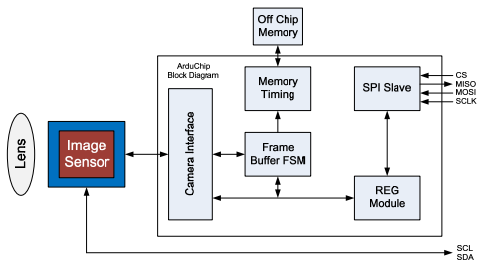
\includegraphics[width=\textwidth]{figures/arducam-block-diagram.png}
        \caption{Architecture of the Arducam Mini 2MP Plus.}
        \label{fig:arducam-block-diagram}
    \end{center}
\end{figure}

\begin{figure}[!htb]
    \begin{center}
        \subfigure[\label{fig:arducam-top}]{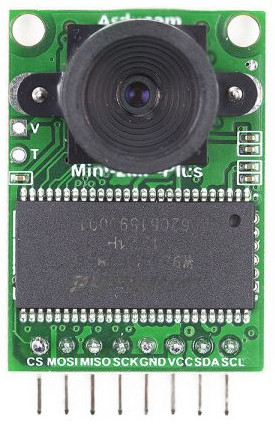
\includegraphics[width=0.16\textwidth]{figures/arducam-top.jpg}}
        ~
        \hfill
        \subfigure[\label{fig:arducam-bottom}]{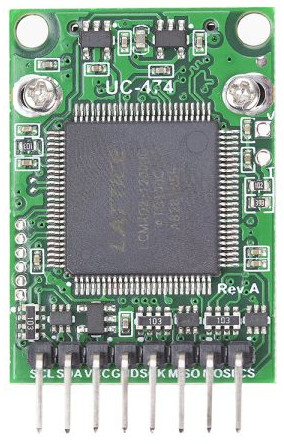
\includegraphics[width=0.16\textwidth]{figures/arducam-bottom.jpg}}
        ~
        \hfill
        \subfigure[\label{fig:arducam-2mp}]{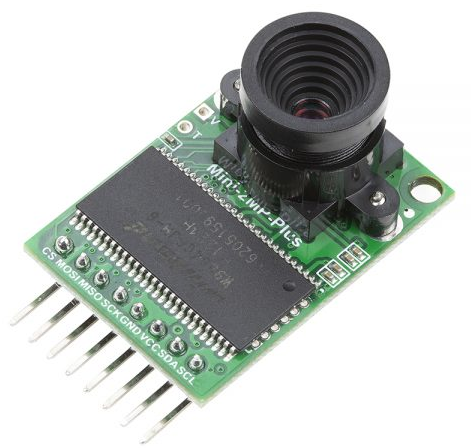
\includegraphics[width=0.3\textwidth]{figures/arducam-2mp.png}}
        ~
        \subfigure[\label{fig:arducam-dimensions}]{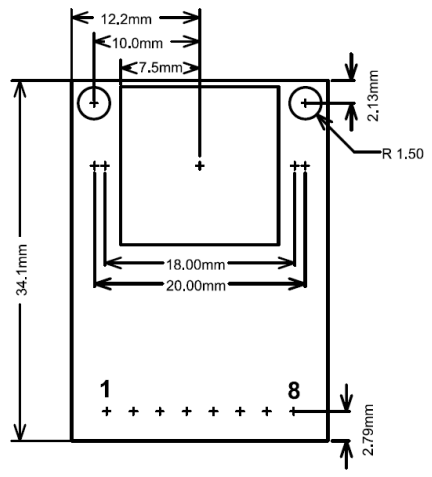
\includegraphics[width=0.3\textwidth]{figures/arducam-dimensions.png}}
        \caption{Arducam Mini 2MP Plus Views and Dimensions.}
        \label{fig:dcp-ex}
    \end{center}
\end{figure}

\section{Electrical Interfaces}

\subsection{Image Sensor Connector}

A connector 1x08 linking all pins from Arducam to the controller.

\subsection{Dedicated Electrical Interfaces}

\textcolor{red}{change images}

\begin{longtable}[c]{lcccl}
    \toprule[1.5pt]
    \textbf{Connector} & \textbf{Image} & \textbf{Interface} & \textbf{Type} & \textbf{Pins} \\
    \midrule
    \multirow{10}{*}{J1} & \multirow{10}{*}{\raisebox{-\totalheight}{\includegraphics[width=4cm]{example-image}}} & \multirow{10}{*}{SPI/Power} & \multirow{10}{*}{PicoBlade} &  \\
                          &  &                           &                            &  \\
                          &  &                           &                            & 3V3 \\
                          &  &                           &                            & GND \\
                          &  &                           &                            & MOSI \\
                          &  &                           &                            & MISO \\
                          &  &                           &                            & CLK \\
                          &  &                           &                            & CS \\
                          &  &                           &                            &  \\
                          &  &                           &                            &  \\
    \midrule
    \multicolumn{5}{r}{\textit{Continues on next page}} \\
    \pagebreak
    \midrule
    \multirow{10}{*}{J3} & \multirow{10}{*}{\raisebox{-\totalheight}{\includegraphics[width=4cm]{example-image}}} & \multirow{10}{*}{JTAG} & \multirow{10}{*}{PinHeade} &  \\
                          &  &                           &                            & \\
                          &  &                           &                            &  \\
                          &  &                           &                            & GND \\
                          &  &                           &                            & 3V3 \\
                          &  &                           &                            & CLK \\
                          &  &                           &                            & DIO \\
                          &  &                           &                            & \\
                          &  &                           &                            & \\
                          &  &                           &                            & \\
    \midrule
    \multirow{10}{*}{CN5} & \multirow{10}{*}{\raisebox{-\totalheight}{\includegraphics[width=4cm]{example-image}}} & \multirow{10}{*}{CAN} & \multirow{10}{*}{PicoBlade} &  \\

                          &  &                           &                            & \\
                          &  &                           &                            &  \\
                          &  &                           &                            & GND \\
                          &  &                           &                            & CAN High \\
                          &  &                           &                            & CAN Low \\
                          &  &                           &                            & \\
                          &  &                           &                            & \\
                          &  &                           &                            & \\
                          &  &                           &                            & \\
    \midrule
    \multirow{10}{*}{CN6} & \multirow{10}{*}{\raisebox{-\totalheight}{\includegraphics[width=4cm]{example-image}}} & \multirow{10}{*}{UART} & \multirow{10}{*}{PicoBlade} &  \\
                          &  &                           &                            & \\
                          &  &                           &                            &  \\
                          &  &                           &                            & GND \\
                          &  &                           &                            & UART\_TX \\
                          &  &                           &                            & UART\_RX \\
                          &  &                           &                            & \\
                          &  &                           &                            & \\
                          &  &                           &                            & \\
    \bottomrule[1.5pt]
    \caption{Dedicated electrical interfaces.}
    \label{tab:icd}
\end{longtable}

\section{Mechanical Interfaces}

\textcolor{red}{TODO}

\section{Controller board}

This section presents some detailed information about the controller board of the SLCam payload, which is a controller designed to integrate with the Arducam in the sattelite.

\subsection{Dimensions}

The controller is a 42.2 $\times$ 25.4 mm board containing four mount holes with 3.2 mm of diameter.

\begin{figure}[!htb]
    \begin{center}
        \subfigure[Top side.\label{fig:arducam-top}]{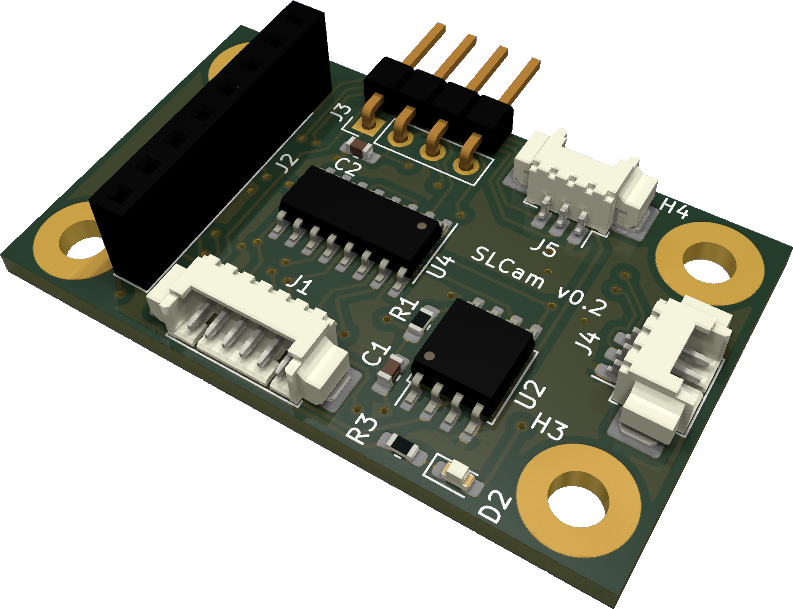
\includegraphics[width=0.45\textwidth]{figures/slcam-overview-top.png}}
        ~
        \hfill
        \subfigure[Bottom side.\label{fig:arducam-bottom}]{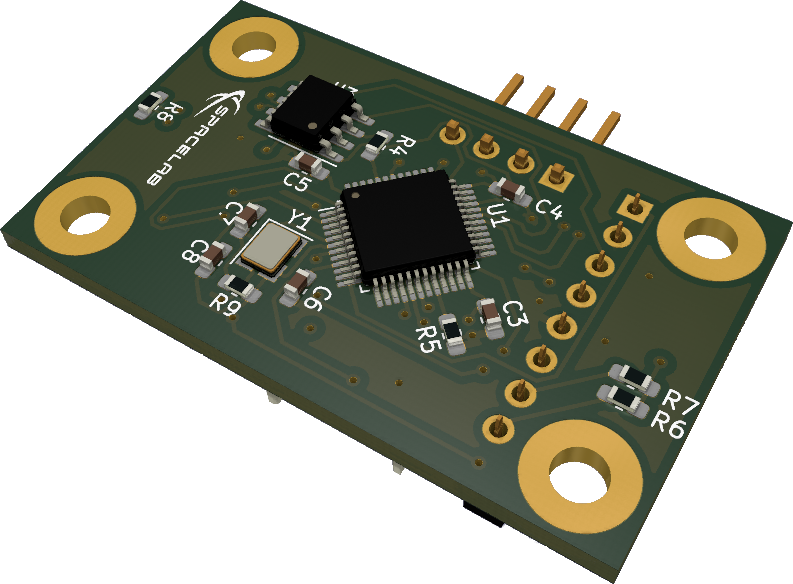
\includegraphics[width=0.45\textwidth]{figures/slcam-overview-bottom.png}}
    \end{center}
        \caption{Top and bottom side of the controller's PCB.}
        \label{fig:slcam-views}
\end{figure}

\subsection{Layout}

The payload was designed with 4 layers \textcolor{red}{as shown in figure x} in the KiCAD v5 software.

It has a thickness of 1.6 mm and surface finish of \textcolor{red}{??}, it was also designe with material \textcolor{red}{??} and it has \textcolor{red}{??} PCB specs. 

\textcolor{red}{put layers photos}

\section{Peripherals}
